% \documentclass{sigchi}

% Use this command to override the default ACM copyright statement
% (e.g. for preprints).  Consult the conference website for the
% camera-ready copyright statement.

% \toappear{Permission to make digital or hard copies of all or part of this work for personal or classroom use is granted without fee provided that copies are not made or distributed for profit or commercial advantage and that copies bear this notice and the full citation on the first page. Copyrights for components of this work owned by others than the author(s) must be honored. Abstracting with credit is permitted. To copy otherwise, or republish, to post on servers or to redistribute to lists, requires prior specific permission and/or a fee. Request permissions from Permissions@acm.org. \\
% {\emph{CHI'16}}, May 07 - 12, 2016, San Jose, CA, USA \\
% Copyright is held by the owner/author(s). Publication rights licensed to ACM. \\
% ACM 978-1-4503-3362-7/16/05...\$15.00 \\
% DOI: \url{http://dx.doi.org/10.1145/2858036.2858529}}

%% EXAMPLE BEGIN -- HOW TO OVERRIDE THE DEFAULT COPYRIGHT STRIP -- (July 22, 2013 - Paul Baumann)
% \toappear{Permission to make digital or hard copies of all or part of this work for personal or classroom use is      granted without fee provided that copies are not made or distributed for profit or commercial advantage and that copies bear this notice and the full citation on the first page. Copyrights for components of this work owned by others than ACM must be honored. Abstracting with credit is permitted. To copy otherwise, or republish, to post on servers or to redistribute to lists, requires prior specific permission and/or a fee. Request permissions from permissions@acm.org. \\
% {\emph{CHI'14}}, April 26--May 1, 2014, Toronto, Canada. \\
% Copyright \copyright~2014 ACM ISBN/14/04...\$15.00. \\
% DOI string from ACM form confirmation}
%% EXAMPLE END -- HOW TO OVERRIDE THE DEFAULT COPYRIGHT STRIP -- (July 22, 2013 - Paul Baumann)

% Arabic page numbers for submission.  Remove this line to eliminate
% page numbers for the camera ready copy 

% \pagenumbering{arabic}

% \usepackage{acmcopyright}

% Load basic packages
% \usepackage{balance}  % to better equalize the last page
% \usepackage{graphicx} % for EPS, load graphicx instead 
%\usepackage[T1]{fontenc}
% \usepackage{txfonts}
% \usepackage{times}    % comment if you want LaTeX's default font
% \usepackage[pdftex]{hyperref}
% \usepackage{url}      % llt: nicely formatted URLs
% \usepackage[usenames,dvipsnames]{xcolor}
% \usepackage{color}
% \usepackage{textcomp}
% \usepackage{booktabs}
% \usepackage{ccicons}
% \usepackage{todonotes}
% \usepackage{xspace}
% \usepackage{amsmath}

% \newcommand{\joschi}[1]{\textcolor{RedOrange}{#1}}
% \newcommand{\adam}[1]{\textcolor{RedOrange}{#1}}

% \newcommand{\joschi}[1]{#1}
% \newcommand{\adam}[1]{#1}

% \newcommand{\eg}{\emph{e.g.}\xspace}
% \newcommand{\etal}{\emph{et~al.}\xspace}

% \newcommand{\prospector}{\emph{Prospector}\xspace}

% \DeclareMathOperator*{\argmin}{arg\,min}
% \DeclareMathOperator*{\argmax}{arg\,max}

% llt: Define a global style for URLs, rather that the default one
% \makeatletter
% \def\url@leostyle{%
%   \@ifundefined{selectfont}{\def\UrlFont{\sf}}{\def\UrlFont{\small\bf\ttfamily}}}
% \makeatother
% \urlstyle{leo}

% To make various LaTeX processors do the right thing with page size.
% \def\pprw{8.5in}
% \def\pprh{11in}
% \special{papersize=\pprw,\pprh}
% \setlength{\paperwidth}{\pprw}
% \setlength{\paperheight}{\pprh}
% \setlength{\pdfpagewidth}{\pprw}
% \setlength{\pdfpageheight}{\pprh}

% Make sure hyperref comes last of your loaded packages, to give it a
% fighting chance of not being over-written, since its job is to
% redefine many LaTeX commands.
% \definecolor{linkColor}{RGB}{6,125,233}
% \hypersetup{%
%   pdftitle={SIGCHI Conference Proceedings Format},
%   pdfauthor={LaTeX},
%   pdfkeywords={SIGCHI, proceedings, archival format},
%   bookmarksnumbered,
%   pdfstartview={FitH},
%   colorlinks,
%   citecolor=black,
%   filecolor=black,
%   linkcolor=black,
%   urlcolor=linkColor,
%   breaklinks=true,
% }

% create a shortcut to typeset table headings
% \newcommand\tabhead[1]{\small\textbf{#1}}

% End of preamble. Here it comes the document.
% \begin{document}

% \CopyrightYear{2016} 
% \setcopyright{acmlicensed}
% \conferenceinfo{CHI'16,}{May 07 - 12, 2016, San Jose, CA, USA}
% \isbn{978-1-4503-3362-7/16/05}\acmPrice{\$15.00}
% \doi{http://dx.doi.org/10.1145/2858036.2858529}

% \title{Interacting with Predictions: Visual Inspection of Black-box Machine Learning Models}

% \numberofauthors{3}

% \author{%
%   \alignauthor{Josua Krause\\
%     \affaddr{New York\\University}\\
%     \affaddr{New York, NY, USA}\\
%     \email{josua.krause@nyu.edu}}\\
%   \alignauthor{Adam Perer\\
%     \affaddr{IBM T.J. Watson\\Research Center}\\
%     \affaddr{Yorktown Heights, NY, USA}\\
%     \email{adam.perer@us.ibm.com}}\\
%   \alignauthor{Kenney Ng\\
%      \affaddr{IBM T.J. Watson\\Research Center}\\
%     \affaddr{Yorktown Heights, NY, USA}\\
%     \email{kenney.ng@us.ibm.com}}\\
% }
% \maketitle

  % UPDATED---\today. Abstracts should be about 150 words and
  % are required.

%%  Understanding predictive models is a challenging task. Often feature importance
%% given by a model is only a rough estimate condensed into one number. Using
%% partial-dependence plots for input features we can visually gain a feeling of
%% how a model is influenced by a given feature. In order to achieve this we treat
%% our machine learning model as a black-box, change our input data slightly, and
%% show the changes of the prediction. Using this technique we gain interesting
%% insights into multiple machine learning models and in turn how to improve them.
%% Furthermore, in the domain of health-care analytics we also use this approach to
%% focus on a single patient. Doing this we can interactively explore how
%% influential features are for a patient. This local importance can be used to
%% identify actionable features where a small change of the patient's state can
%% lead to a significant change of the disease risk of this patient.

% kng: I reworded the abstract ... feel free to not use if you don't like it
\begin{quote}\textit{
Understanding predictive models, in terms of interpreting and identifying actionable
insights, is a challenging task.
Often the importance of a feature in a model is only a rough estimate
condensed into one number.  However, our research goes beyond these na\"ive estimates through the design and implementation of an interactive visual analytics system,
\prospector. By providing interactive partial dependence diagnostics, data scientists can understand how features affect the prediction overall.  In addition, our support for localized inspection allows data scientists to understand how and why specific instances are predicted as they are, as well as support for  tweaking feature values and seeing how the prediction responds.  Our system is then evaluated using a case study involving a team of data scientists improving predictive models for detecting the onset of Diabetes from electronic medical records.
}\end{quote}
% Using partial-dependence plots provides a way to visualize how a model
% is influenced by a given feature.
% This is achieved by treating the machine learning model as a black-
% box, systematically changing the input data values, measuring and
% then showing the changes in the prediction score.
% Using this technique, insights into multiple machine learning models
% can be obtained which can then in turn be used to improve them.
% Furthermore, in the domain of health-care analytics, this approach can
% be used to focus on a single patient. Specifically, one can
% interactively explore how influential different features are for an
% individual patient. This local importance can be used to identify
% actionable features where a small change in the patient’s state can
% lead to a significant change in the patient's predicted risk.

\begin{contributions}{How can partial dependence be leveraged to gain diagnostic insights into machine learning models?}
\item The partial dependence based feature importance score allows to effectively detect model errors.
\item Detectable errors include: over-fitting, under-fitting, biases in the data caused by imputation, and leaking labels caused by incorrect cause-effect relationships.
\item Localized inspections help to understand the how and why of specific instance predictions by finding locally impactful features.
\end{contributions}

\begin{quote}
\textit{Josua Krause, Adam Perer, Kenney Ng}
\end{quote}

% \keywords{interactive machine learning; predictive modeling; partial dependence; %\joschi{sensitivity analysis;}
% visual analytics; model visualization}

% \category{H.5.m.}{Information Interfaces and Presentation
%   (e.g. HCI)}{Miscellaneous}
   % \category{See
  % \url{http://acm.org/about/class/1998/} for the full list of ACM
  % classifiers. This section is required.}{}{}

% !TEX root = ../prospector.tex

% \section{Introduction}

In the era of data-driven analytics, there is growing demand to generate and deploy predictive models in a variety of domains so that the patterns unearthed from massive amounts of data can be leveraged
% for the greater good.
and converted into actionable insights.
Predictive modeling is defined as the process of developing a mathematical tool or model that generates an accurate prediction \cite{kuhn2013applied}.  As an example, in health care, if one can model the data characteristics of patients who will likely develop Diabetes, health care institutions could deploy such a model on their patient databases, and automatically flag high risk patients to clinicians to make sure they are being treated appropriately.  However, building such models on noisy, real-world data is quite challenging.  

Data scientists often turn to machine learning, where the goal is to create predictive models based on information automatically learned from data with ground truth.  However, these machine learning techniques are often black-boxes and may be selected based only on performance metrics such as high accuracy scores, and not necessarily based on the interpretability and actionable insights of the model.  There has recently been a variety of techniques to inject humans-in-the-loop when building predictive models based on machine learning, from interactive training \cite{amershi15} to interactive feature selection \cite{infuse}.  However, interactive systems to effectively assess and evaluate the interpretability and actionable insights of a predictive model that go beyond simple accuracy metrics is still lacking.  We believe bringing humans into the loop at this stage can possibly lead to better models and consequently improved outcomes when the models are deployed.

Our research aims to support data scientists to go beyond judging predictive models solely based on their accuracy scores by also including model interpretability and actionable insights.  Towards this goal, we developed \prospector, a novel visual analytics system designed to help analysts better understand  predictive models.  \prospector leverages the concept of partial dependence, a diagnostic technique that was designed to communicate how features affect the prediction, and makes this technique fully interactive.  \prospector also supports localized inspection, so users can understand why certain data results in a specific prediction, and even lets users hypothesize new data by tweaking values and seeing how the predictive model responds.  We also demonstrate, through a case study, how the system can lead to important insights for clinical researchers building models that try to predict patient outcomes based on electronic medical records.

Concretely, our contributions include:

\begin{itemize}
\item A design and implementation of an interactive visual analytics system,
\prospector, for assessing the interpretability and actionable insights of trained predictive models by supporting:
\begin{itemize}
    \item Interactive partial dependence diagnostics to understand how features affect the prediction overall. There are novel visual representations, sampling strategies, and support for comparing multiple models.
    \item Localized inspection to understand how and why specific instances are predicted as they are.  Users can interactively tweak feature values and see how the prediction responds, as well as find the most impactful features using a novel local feature importance metric.
  \end{itemize}
\item A case study of data scientists using
\prospector to improve predictive models for detecting the onset of Diabetes trained from electronic medical record data.
\end{itemize}

% \begin{itemize}
%   \item Machine learning algorithms increasingly being relied on in data science.
%   \item One such class of machine learning algorithms are predictive classifiers.
%   \item Predictive models offered judged by their accuracy score, and not necessarily by their components.
%   \item For those examining components, judgment is often done via naive importance weights
%   \item Our contribution is to go beyond these naive metrics to provide:
%   \begin{enumerate}
%     \item Partial Dependence.  Understand how features affect the prediction overall.  Leverage an existing diagnostic technique called partial dependence, but make it interactive/coordinated.
%     \item Localized Inspection.  How does the model affect specific data rows (patients).
%   \end{enumerate}
%   \item Deeper inspection of predictive models can help ensure the models are grounded in reality.
%   \item Help data scientists focus on determining actionable features (to go beyond prediction) e.g. focusing clinicians on features that may improve the patient's health, or focusing city managers on features that may lower crime.
% \end{itemize}

% Theme of 2016 conference is \#chi4good.  Play up how bringing humans in the loop for important domain predictions can possibly lead to better models and better outcomes.

% Two parts:
% 1. what are partial dependence plots good for? (global)
% its useful for inspecting and improving models.
% 2. how to use partial dependence for predicting single rows (local)
% its also useful as a local tool for understanding the impact of the model on specific data points.

% !TEX root = ../prospector.tex

\section{Motivation}

\subsection{Machine Learning for Predictive Modeling}

Data scientists often use machine learning to create predictive models based on known properties of  training data, which acts as the ground truth. 
%Predictive modeling is a machine learning discipline that uses observed data to predict unobserved outcomes.
%Often classification is used that instead of having a numeric outcome like risk has a few categories.
%Numeric outcomes can always be converted into categories.
%For example risk can be categorized into low, medium, and high risk.
Machine learning algorithms typically work in two phases: the training phase and the prediction phase.
In the training phase, parameters of the model are
learned using training data.
%In the training phase, outcomes from training data are used to verify the quality of prediction and make changes to internal values of the model until a local maximum is reached.
% Typically unstructured data is converted into feature vectors to be usable with common machine learning algorithms.
The prediction phase then computes predictions using the trained model. % The model does not change in this phase anymore.
Below, we describe several machine learning algorithms that are commonly used and also utilized in the case study.

A decision tree is one such algorithm, which is a tree whose nodes are rules that decide how to proceed down the branches of the tree, according to the range of values for a specific feature.  The decision making starts at the root of the tree and leaves carry the prediction results. Decision trees are popular in machine learning as they allow data scientists to model arbitrary functions.
However, the more nodes a tree has, the harder it is to understand the reasoning behind outcomes.
Logistic regression is another popular algorithm that is easier to understand, as features can only positively or negative influence the prediction, and the rate of influence is fixed.  This is achieved by defining a hyper-plane in the feature vector space, where the outcome of the prediction depends on how close to and on which side of the hyper-plane an instance is.

% Each feature contributes linearly to the outcome.
% So a low value of a feature leads to a low outcome and a high value to a high outcome or a low value leads to a
% high outcome and a high value to a low outcome.
% Each feature is assigned one weight that determines how rapid changes in the value change the outcome.

Another popular algorithm is random forests, which combine the output of multiple decision trees.
A random forest is an example of an ensemble model, which combines the output of several weak machine learning models to yield an overall better result with less bias and variance than a single strong model.
% Random forest is an example of a boosting model, which works under the assumption that combining the output of several weak machine learning models yield an overall better result than a single strong model.
However, this makes ensemble models less interpretable since each weak model has only a small influence on the outcome.
% Random forests are boosting models consisting of decision trees that are built using randomized thresholds that are improved during the training phase.  Randomization is necessary since otherwise all trees would be identical.


\subsection{Predictive Modeling in Health Care}

In order to make our contributions concrete, we utilize a motivating scenario that emerged from our case study.  The case study involves a team of five data scientists interested in using predictive modeling on a longitudinal database of electronic medical records. The research team has a background in health care analytics and their database contains 4,000 patients from a major hospital in the United States. The team is interested in building a predictive model to predict if a patient is at risk of developing Diabetes, a chronic disease of high blood sugar levels that may cause serious health complications.

% !TEX root = ../prospector.tex

\begin{figure}
\centering
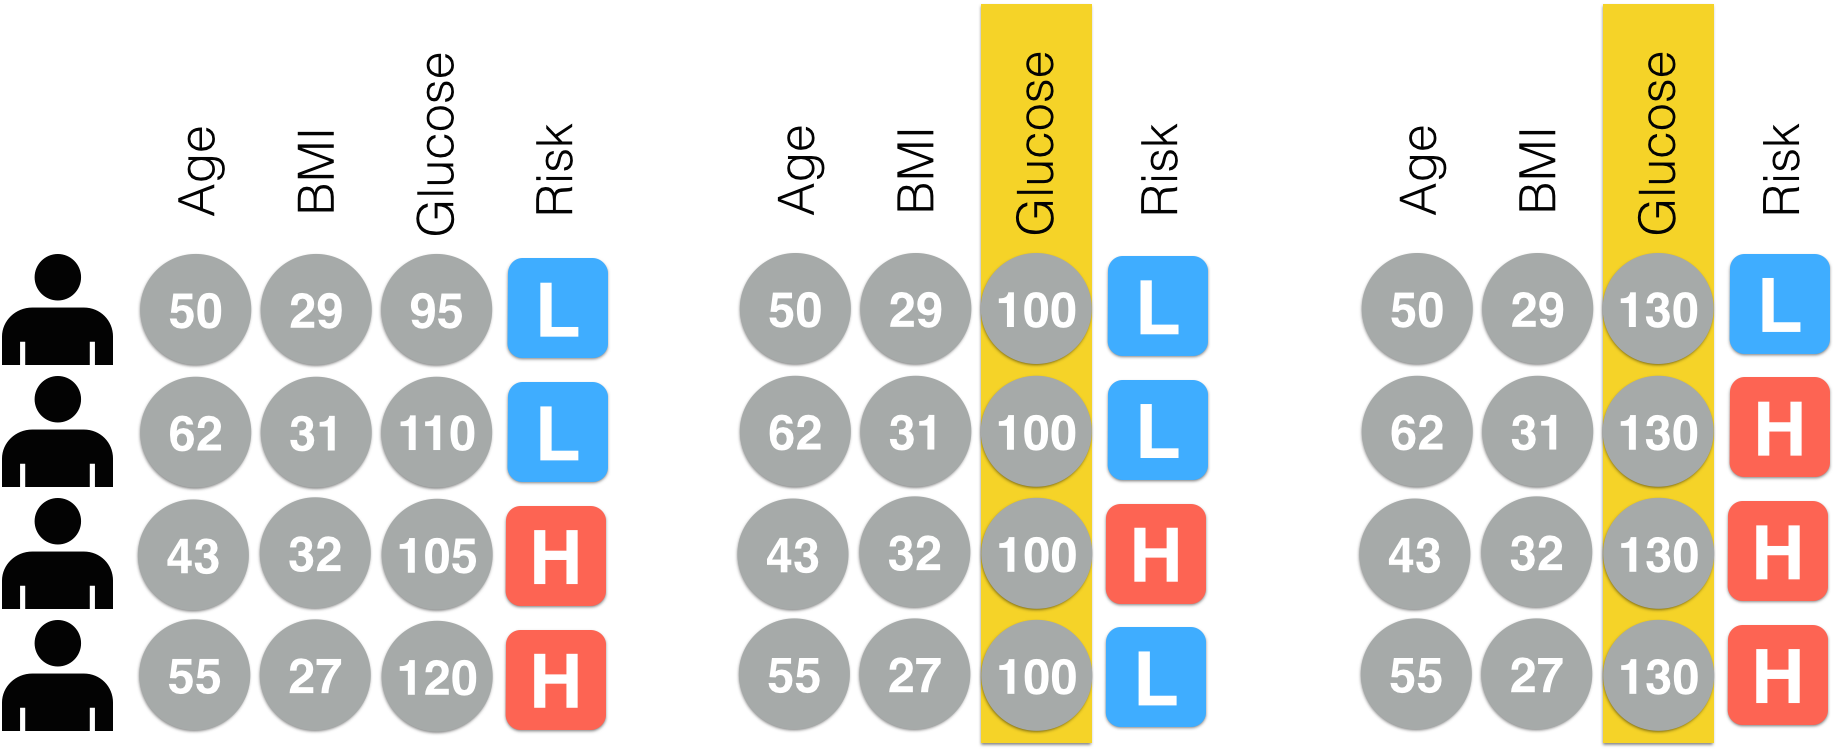
\includegraphics[width=0.90\linewidth]{prospector/partial-dependence-explanation} % 0.95
\caption{
An illustration of how partial dependence is computed for the feature ``Glucose".  On the left are four patients' original feature values.  In the middle, the ``Glucose" values are all changed to 100, and the corresponding predictions change.  Similarly, on the right, the ``Glucose" values are all changed to 130, and again the risks are different.  This demonstrates the impact of the ``Glucose'' feature on risk prediction.
% The plotted value in a Partial Dependence plot is the average of the
% ``Risk" probability values.
}
\label{figs:pdexplain}
\end{figure}

The team of data scientists manages to develop a highly accurate predictive model for detecting patients at high risk of developing Diabetes.  They determine its effectiveness by measuring the common metrics used by predictive models (e.g., accuracy and AUC scores \cite{kuhn2013applied}).  They also followed the best practices of building predictive models.  They worked with clinical researchers to properly define cohorts of patients with Diabetes (cases) and matched patients without Diabetes (controls) by thoroughly searching through the electronic medical records.  They constructed features based on lab tests, diagnosis codes, procedures, demographics, and patient conditions from the records.  They used cross-validation to ensure their models were robust.  They used a variety of state-of-the-art feature selection methods to utilize the most informative features in the model while keeping it as generalizable as possible.  And they used a variety of effective classifiers to do the training and evaluation.  After trying various combinations of these techniques, the model with the highest accuracy metrics was selected and presented to the appropriate stakeholders at the health care institution.

Their stakeholders were impressed by the high accuracy scores of the model.  But when they asked the data scientists for more information about what was inside of the model, the reports only described the top features of the model and their associated ``importance" weights.  The stakeholders recognized many of the feature names, and it appeared to make clinical sense.  However, there were also some surprising ones that led to intellectual discussions.  But the stakeholders demanded to know more.  They wanted a clearer sense of how certain features impacted the prediction.  Furthermore, they wanted to understand how the values associated with the features (\eg, the results associated with lab tests) impacted the prediction.  They also were curious to interact with the model to test hypotheses about how the model would react to hypothetical patients of interest.  When confronted with these questions, the data scientists shrugged.  In the data scientist's defense, it is difficult to summarize and interpret complex models and there are few tools and techniques available to address the stakeholders' requests.  So now the stakeholders are faced with a hard decision:  do they deploy a predictive model in their institution that appears to have high accuracy but is also somewhat of a black-box?

Although this scenario is motivated by our case study, our other projects and interviews suggest these are not atypical requirements.  Our work is motivated to support the development of more comprehensible predictive models. 

\subsection{Partial Dependence}

% !TEX root = ../prospector.tex

\begin{figure}[t]
\centering
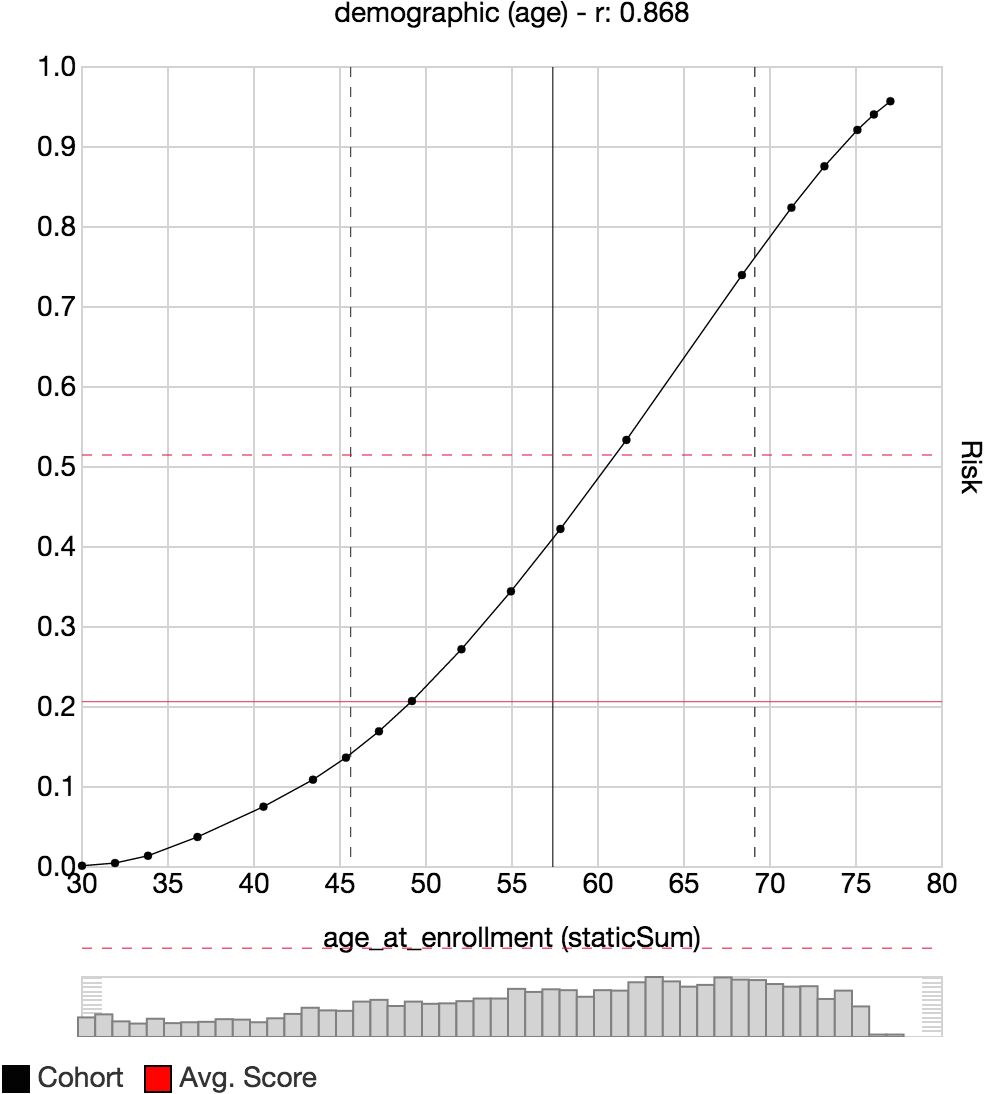
\includegraphics[width=0.55\linewidth]{prospector/pdp_reg} % 0.7
\caption[Partial dependence plots.]{
Partial dependence plots. The black curve shows the average predicted risk
(probability of a certain outcome) if for all rows in the data the value of this
feature was the given value of the horizontal axis.
The red line shows the average predicted risk for the original data.
The vertical line shows the mean of the observed values and the histogram below the plot
shows the distribution of observed values.
Dotted lines show the range of one standard deviation around the mean values.
}
\label{figs:pdp}
\end{figure}

The most widely used technique to understand the relationship between a feature and a prediction is by computing partial dependence \cite{friedman2001,hastie2001}.
The idea of partial dependence plots is to treat predictive models as a black-box and observe how changes in the input affect prediction outcomes.
When inspecting only the partial dependence of one input feature at a time, Formula (\ref{eq:pdp}) can be used to compute a partial dependence plot.

\begin{equation}
pdp_f(v) = \frac{1}{N} \sum_i^N pred(x_i) \;\text{with}\; x_{if} = v
\label{eq:pdp}
\end{equation}

$N$ is the number of rows in the input matrix $x$,
$pred$ is the prediction function that takes one input row, a feature vector, and returns an outcome probability,
and $f$ is the feature used to compute the partial dependence plot.
The formula computes the average outcome over all input rows while changing the value of feature $f$ to the
input value $v$ for each row $x_i$. The original input data is kept fixed. This allows for observing the influence of $f$
on the predicted probabilities.

In order to make this function more concrete, consider the illustrative example in Figure~\ref{figs:pdexplain}, where each input row is a patient, and each column is a feature.  The last column represents the output of the predictive model that predicts if a patient is at low-risk or high-risk for developing Diabetes.  In Figure~\ref{figs:pdexplain}a, the patients' original feature values (age, BMI (Body Mass Index, a standard way to quantify obesity), and glucose level (a standard way to determine Diabetes)) are shown.  If one wants to examine the impact of the glucose feature on the prediction, partial dependence can be applied by keeping all of the other features (age, BMI) as they were, but fixing glucose to a set of fixed values to see how that feature impacts the prediction.  For example, in Figure~\ref{figs:pdexplain}b, the glucose values (highlighted in yellow) are fixed to 100, which yields predictions of only 1 patient being high risk, instead of the original 2.  Conversely, in Figure~\ref{figs:pdexplain}c, glucose is fixed to 180, and 3 patients are predicted to have high risk.  Thus, there appears to be partial dependence of glucose on the prediction.  

Partial dependence is typically visualized as a partial dependence plot, as shown in Figure~\ref{figs:pdp}, which is a line graph that plots the fixed values of the target feature on the x-axis, and the corresponding predicted risk (\ie, probability of a certain outcome) on the y-axis.  


% !TEX root = ../prospector.tex

\section{Related Work}

\subsection{Motivation for Interpretability}
Modern machine learning algorithms are able to create more reliable and precise models
but they are increasingly complex and come with the price of being harder and harder to interpret (Breiman~\cite{breiman2001}).
This inverse relation of understandability versus expressiveness of a model introduces the need
to find ways to improve the interpretability of complex models to overcome this disadvantage.
Lim~\cite{Lim:2012:IUT:2518922} asks questions such as ``\emph{Why} did X happen?",
``\emph{Why} not Y?", ``\emph{What} happens \emph{if} I do Z?", and ``\emph{How} do I make X happen?"
to explain complex mechanisms like machine learning models.
Our system allows users to interactively ask and answer such questions.
Kulesza~\etal~\cite{Kulesza:2015:PED:2678025.2701399} use explanatory debugging by conveying how a model
came to its prediction in order to be able to correct mistakes.
On the other hand, Patel~\etal~\cite{DBLP:conf/ijcai/PatelDFKT11} use multiple classifiers
to better understand input data.
Steeg~and~Galstyan~\cite{NIPS2014_5580,steeg2015corex_theory} use total correlation to build
a hierarchy of features explaining their role in the data.

\subsection{Algorithm Specific Model Visualization}
In the past, research has primarily focused on understanding and interacting with specific machine learning algorithms.
Often the focus is on the internal weights of the trained models.
For Bayesian networks, showing probabilities of the nodes (Becker~\etal~\cite{Becker:2001:VSB:383784.383809}) and how the input is propagated (Correa~\etal~\cite{DBLP:journals/isci/MartinsONHC13})
has been used.
For Support Vector Machines,
projection techniques (Caragea~\etal~\cite{Caragea2001}) and
Nomograms (Jakulin~\etal~\cite{Jakulin:2005:NVS:1081870.1081886})
to see the ``cut" in the data points were utilized.
Visualizing and interpreting the graph of a neural network has also been used by Tzeng and Ma~\cite{Tzeng:2005:OTB}.
Kim~\etal~\cite{kim2014bayesian,kim2015MGM} introduce graphical models that allow for
interpretability of its features.
\cite{kim2015MGM} use a colored matrix of features by category to show distinguishable features computed by their model.
Caruana~\etal~\cite{Caruana:2015:IMH:2783258.2788613} use high-performance generalized additive models (GA$^2$Ms) that allows visual inspection of the influence of its input features on the outcome much like partial dependence.

\subsection{Model Result Visualization}
However, showing only internal, algorithm specific weights is often not enough.
Plate~\etal~\cite{DBLP:journals/neco/PlateBGB00} and Olden~\cite{citeulike:3733836} show how input features influence
the outcome of neural network classifications.
Xu~\etal~\cite{DBLP:journals/corr/XuBKCCSZB15} interprets
the graph of a neural network used for image classification to
retrieve which part of an image was responsible for a specific
classification result.
These techniques aim in the same direction as partial dependence but are limited to only neural networks.
They cannot be used to support the ability to compare different machine learning models across algorithms.

Having access to the internals of a machine learning algorithm also allows direct interaction with the models and to improve them on the fly.
BaobabView (van den Elzen and van Wijk~\cite{6102453}) offers interactive decision tree construction.
Steed~\etal~\cite{5332586,doi:10.1559/152304009788988314}
guides regression model creation by enhancing interaction
with the input data.
EnsembleMatrix (Talbot~\etal~\cite{Talbot:2009:EIV:1518701.1518895})
allows users to combine already computed classification models to
build ensemble models.
Some recent interactive machine learning tools \cite{
amershi15,
Amershi:2011:DEE:2046396.2046416,
Amershi:2012:RIM:2207676.2207680,
Amershi:2011:CHF:1978942.1978966,
Kapoor:2010:IOS:1753326.1753529,
kim2015scalable,
Leung2014710,
Mishra:2015:SAI:2700171.2791022,
export:141330})
are more algorithm agnostic, but depend on general
performance measures like confusion matrices,
area under ROC curve (AUC) measures,
result distribution of data points, and
feature weights according to model independent statistics.

Frank and Hall~\cite{frank2003} use 2D projections of the data to show %classification
results for multiple classification algorithms, as well as Rheingans and desJardins~\cite{885740} with self-organizing maps.

\subsection{Probing Models}
Partial dependence was proposed by Friedman~\cite{friedman2001} for analyzing
gradient boosting models and has since been used for other models as well (\eg Ehrlinger~\cite{ehrlinger2015} uses partial dependence to analyze the behavior of random forests
in the \emph{R} package \emph{ggRandomForests}).

Cortez and Embrechts~\cite{cortez2011opening,Cortez20131} and Kim~\etal~\cite{kim2014bayesian}
use sensitivity analysis to analyze and compare machine learning models of different algorithms.
Sensitivity analysis is similar to partial dependence except that it uses a few
base vectors (usually the mean, median, or quartiles of all observed values)
instead of computing the probabilities over all input points.
This method is faster than partial dependence but may miss critical details
about the prediction function especially if the function is strongly non-linear.

Goldstein~\etal~\cite{goldstein14} extends the idea of partial dependence by using
Individual Conditional Expectation (ICE) plots which show one line for each row of the input data.
We found, however, that this often clutters the plots too much and makes them harder to interpret.
We experimented further with showing standard deviations and quartiles of the partial dependence line
but discarded this approach since the spread of the partial dependence results is always expected to
be large unless one feature dominates the classification significantly and is able to solely change
the classification even for the furthest data points.

By not restricting ourselves to sampling only the observed input space, our approach on partial dependence
enables a deeper analysis of the machine learning model. Furthermore, accepting the costs of computing
partial dependence over all input points yields proper results even for highly non-linear models,
while also not overwhelming users with too much detail.
This is strengthened even further by our novel approach of using implementation details of the inspected
models to improve the sampling and the representation of the results.

% !TEX root = ../prospector.tex

\begin{figure}[t]
\centering
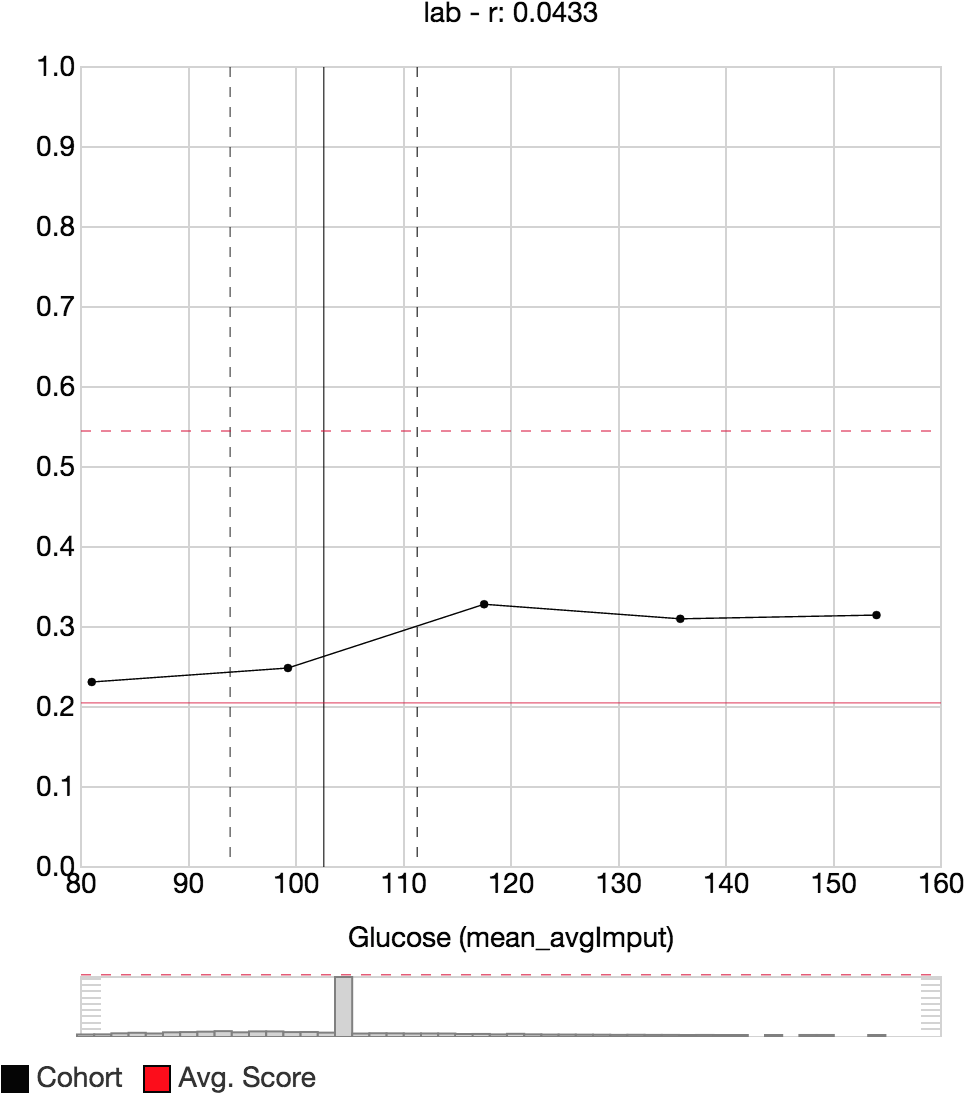
\includegraphics[width=0.3\textwidth]{prospector/sampling_1} % 0.3
~
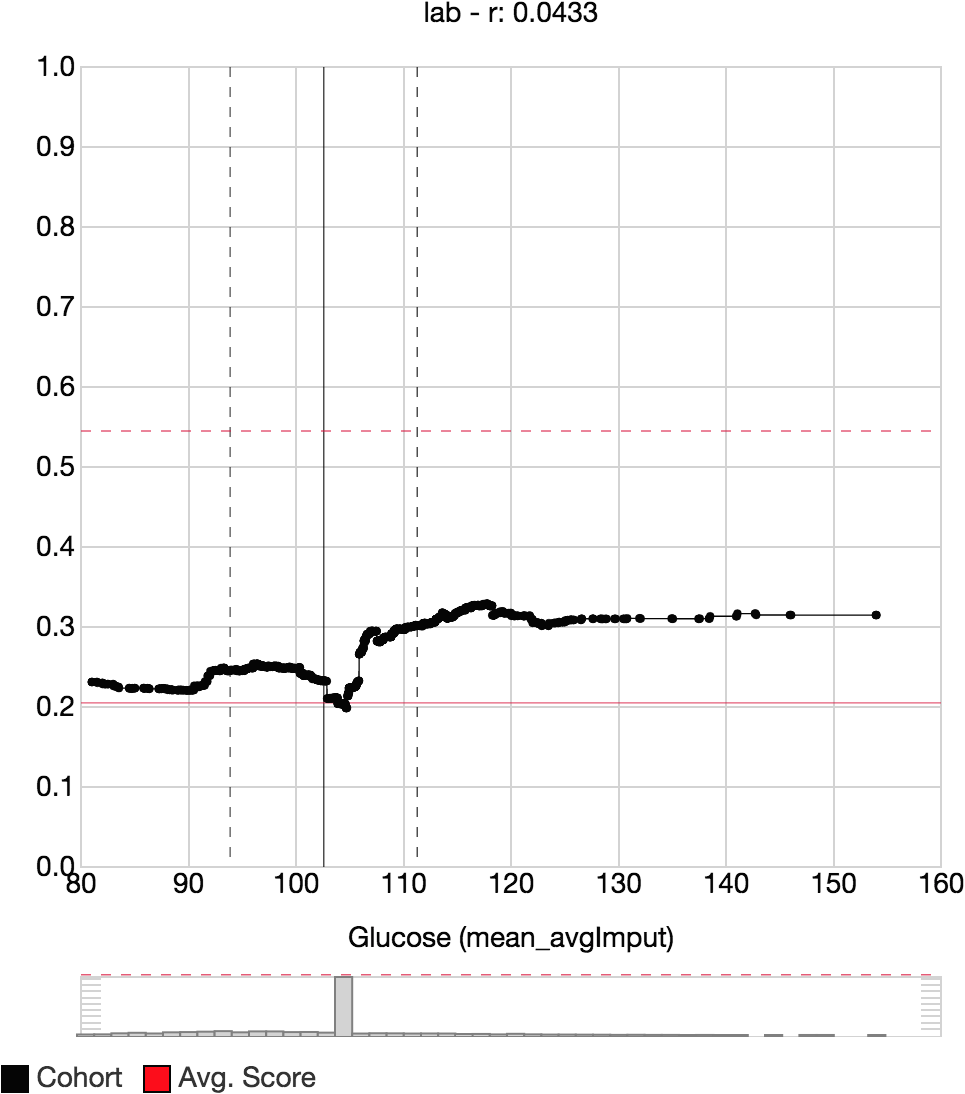
\includegraphics[width=0.3\textwidth]{prospector/sampling_2} % 0.3
~
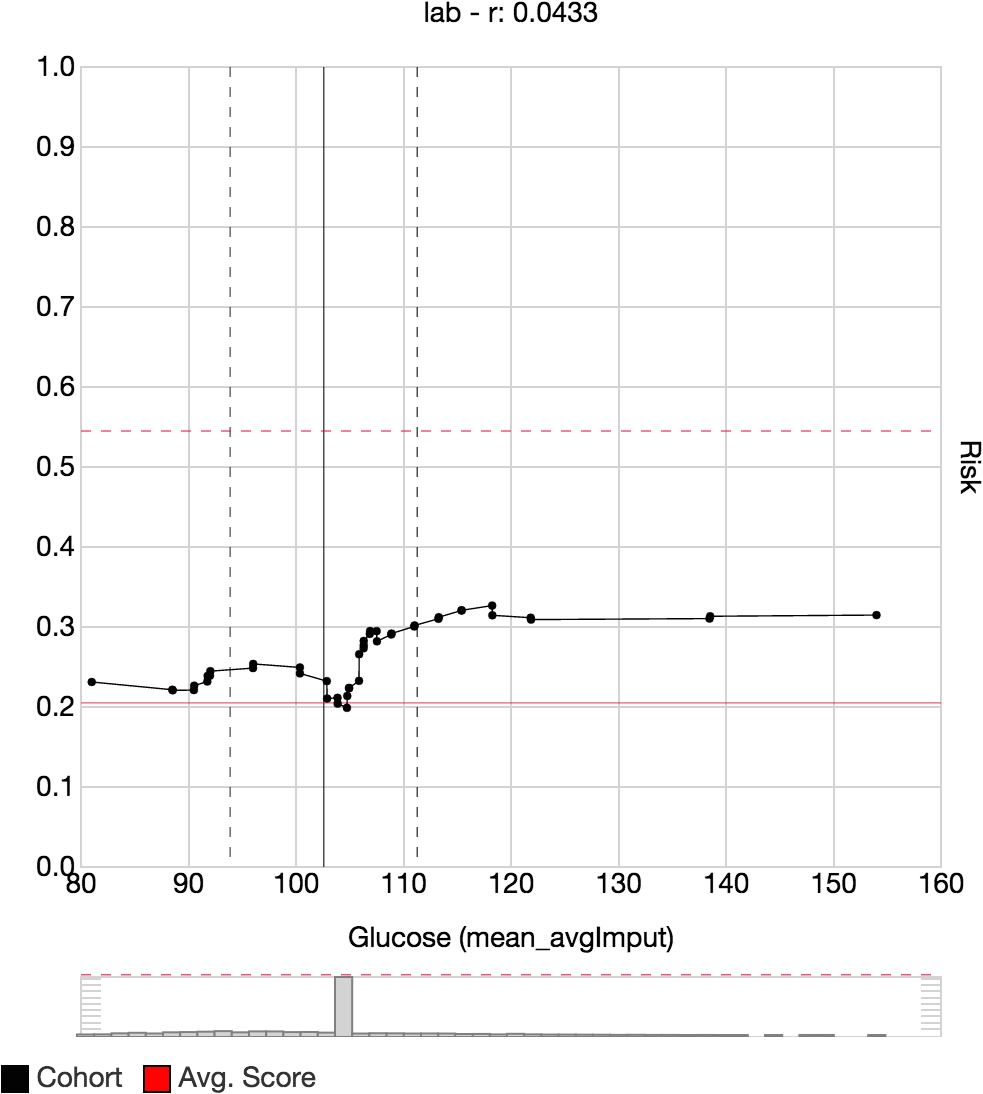
\includegraphics[width=0.3\textwidth]{prospector/sampling_3} % 0.3
\caption[Different sampling strategies for partial dependence plots.]{
Different sampling strategies for partial dependence plots.
The leftmost plot uses a na\"ive sampling which misses the
dip in the predicted risk for a Glucose value around 105.
Using the thresholds of the trees in the random forest
the middle plot shows all details of the displayed model.
The rightmost plot simplifies this by detecting co-linear points
and summarizing them into lines improving readability.
The dip in the predicted risk is due to imputation of missing values
to the mean of the observed values.
This increase in local noise shifts the prediction towards the overall
average predicted risk (the horizontal red line).
Most patients have never had their Glucose value measured.
}
\label{figs:sampling}
\end{figure}

\section{System}
In order to integrate partial dependence and localized inspection into our pipeline we propose
\prospector, a web-based interface.  The server side of \prospector can load any machine learning model accessible via python, or integrate with existing predictive modeling pipelines such as PARAMO \cite{paramo}.
% This can be done via a special admin page in the UI which also allows to
% precompute some partial dependence plots.
Although this paper demonstrates the system on clinical data, the tool is able to handle predictive models for other domains.  For example, the tool has also been used with exploring models that predict real estate prices, as well as classic data sets from the UCI Machine Learning Repository \cite{Lichman:2013}.

In this section, we first describe \prospector's novel enhancements of partial dependence plots.  Then, we describe how \prospector leverages partial dependence to support localized inspection.  Finally, we describe the workflow of how these techniques are integrated into \prospector's UI.
\subsection{Partial Dependence Plots}

Partial dependence is typically visualized as a partial dependence plot, which is a line graph that plots the fixed values for the target feature on the horizontal axis, and the corresponding predicted risk (probability of a certain outcome) on the vertical axis.  In \prospector, we enhance the plot by adding a red reference line with the average predicted risk of the model on the original data, as shown in Figure~\ref{figs:pdp}.  In addition, a black vertical line indicates the average observed value of the input data for the current feature.  Both reference lines are accompanied with dotted lines showing one standard deviation in both directions from the  mean value.  To help with validating insights and assigning importance, a histogram of the observed values in the original data is also shown below the plot.

\subsubsection{Sampling Partial Dependence}

% \adam{BE CLEAR INSPECTING PD is OUR CONTRIBUTION.}

One of our core contributions is the ability to effectively treat partial dependence as a black-box for inspection.  However, na\"ively treating the predictive model as black-box may lead to inaccuracies in the generated plot.
Often only observed input values are used for sampling which leaves the prediction
function for other values undefined, even though those values might be of
particular interest for understanding the internals of the model.
Furthermore, the interpolation between those sample points may ignore inherent
features of the prediction function.
For example, Ehrlinger~\cite{ehrlinger2015} shows the usage of
partial dependence plots via random forest models.
The prediction function for those models can only change between thresholds
appearing in the nodes of the trees.
For all other values the prediction remains constant.
However, the interpolation between sample points used in the examples
is polynomial.
This leads to the following misrepresentations of the prediction function:
\begin{itemize}
\item Some sampled prediction values are not included in the interpolation.
\item The interpolation is a curve where it should be a constant which alludes to values that are impossible to achieve with the prediction function.
\item Steps are interpolated as curves which gives the impression of a smooth ascent of values when it should be a series of sudden jumps.
\end{itemize}

We overcome those inaccuracies by acknowledging inherent properties of
the prediction functions of our models.
This is only possible by leveraging the internal design of model algorithms and
therefore, \prospector must more effectively sample the range of the input features.
For example, in decision tree or forest models, where the predicted risk will not change between thresholds of the nodes of those models' trees
\prospector utilizes the knowledge that the plot will be a step function by only sampling values at the thresholds of the given feature to accurately
compute the complete plot (see Figure~\ref{figs:sampling}).
It does this by inspecting the decision rules in the nodes of the model to retrieve those thresholds.

However some models, such as random forest models, produce a large number of points
where the outcome might change which leads to a cluttered plot that impairs readability.
One solution to this is to simplify the generated plot by finding almost co-linear points and reducing them to the end-points.
Such visual optimizations support more comprehensible plots that are easier to read while still being accurate representations. Other machine learning algorithms may not require such optimizations.

\prospector also enhances partial dependence plots by taking into account the context of the original data values.  For example, certain features only make sense as integer values (\eg, the number of times a laboratory test was performed) and it does not make sense to show non-integer values in the plots.
Such features can be heuristically detected by inspecting the set of values in the original data set and \prospector restricts those features to only have integer values as input.
Similarly, in the partial dependence plot, only integer values are computed.
Furthermore, for predictive models using step functions the plot
is horizontally shifted by $0.5$ so that jumps happen between values.
This eases reading the actual value at the integer points.
Even though this improvement leads to a slight misrepresentation of the prediction function for non-observable values the readability of the plot is significantly improved to support user tasks.
For non-integer data types, these optimizations are not necessary.

\subsection{Local Inspection}
% !TEX root = ../prospector.tex

% !TEX root = ../prospector.tex

\begin{figure}[b!]
\centering
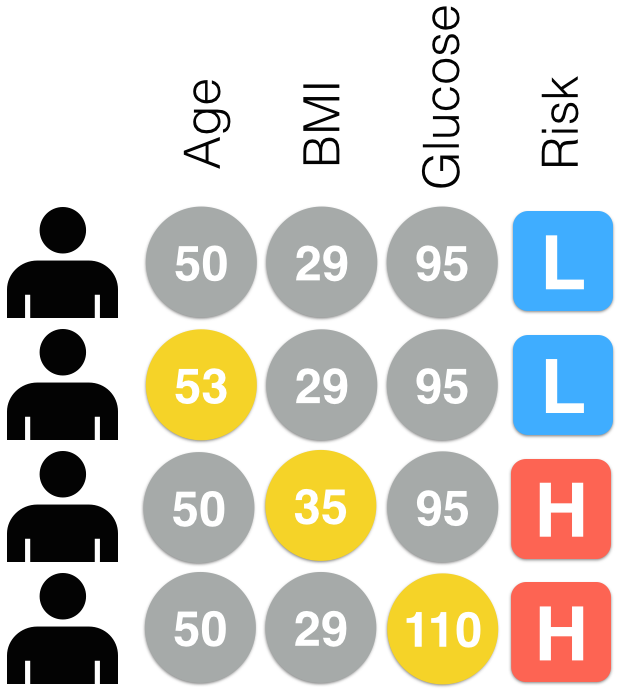
\includegraphics[width=0.3\linewidth]{prospector/local-inspection-explanation} % 0.3
\caption{
This illustration provides an explanation of how local inspection works.  On the top row are the patient's original feature values and the corresponding prediction.  On the bottom three rows, users changed certain values of the patient, highlighted in yellow, and such values impacted the prediction.
}
\label{figs:liexplain}
\end{figure}

Our second core contribution is leveraging our implementation of partial dependence to support the user task of local inspection.  Users can use \prospector to inspect specific data points of interest and see how the models predict how they behave.  In addition, if the users are curious about how a particular data point's risk might change if it had different values, a user can explore this as well.  The idea of localized inspection is illustrated in Figure~\ref{figs:liexplain} using our running example of Diabetes prediction.  At the top, the original patient's feature values are shown, along with the patient's original predicted low risk of having Diabetes. Suppose the analyst was curious to see how the patient's risk would change if his BMI was increased to 35.
Localized inspection allows users to interactively change this value, and see the corresponding prediction.
In order to streamline this kind of exploration we fully compute the
predicted risk for all values of BMI similar to partial dependence.
As seen in Figure~\ref{figs:liexplain} we do this for all features independently
yielding local partial dependence plots for each feature using a single input row.
% Using the idea of partial dependence on a single row of the input data set creates a localized partial dependence describing the axis aligned neighborhood of one point in the prediction function. This enables what-if scenarios by changing some values of the input row and seeing how the predicted outcome changes.

\begin{figure}
\centering
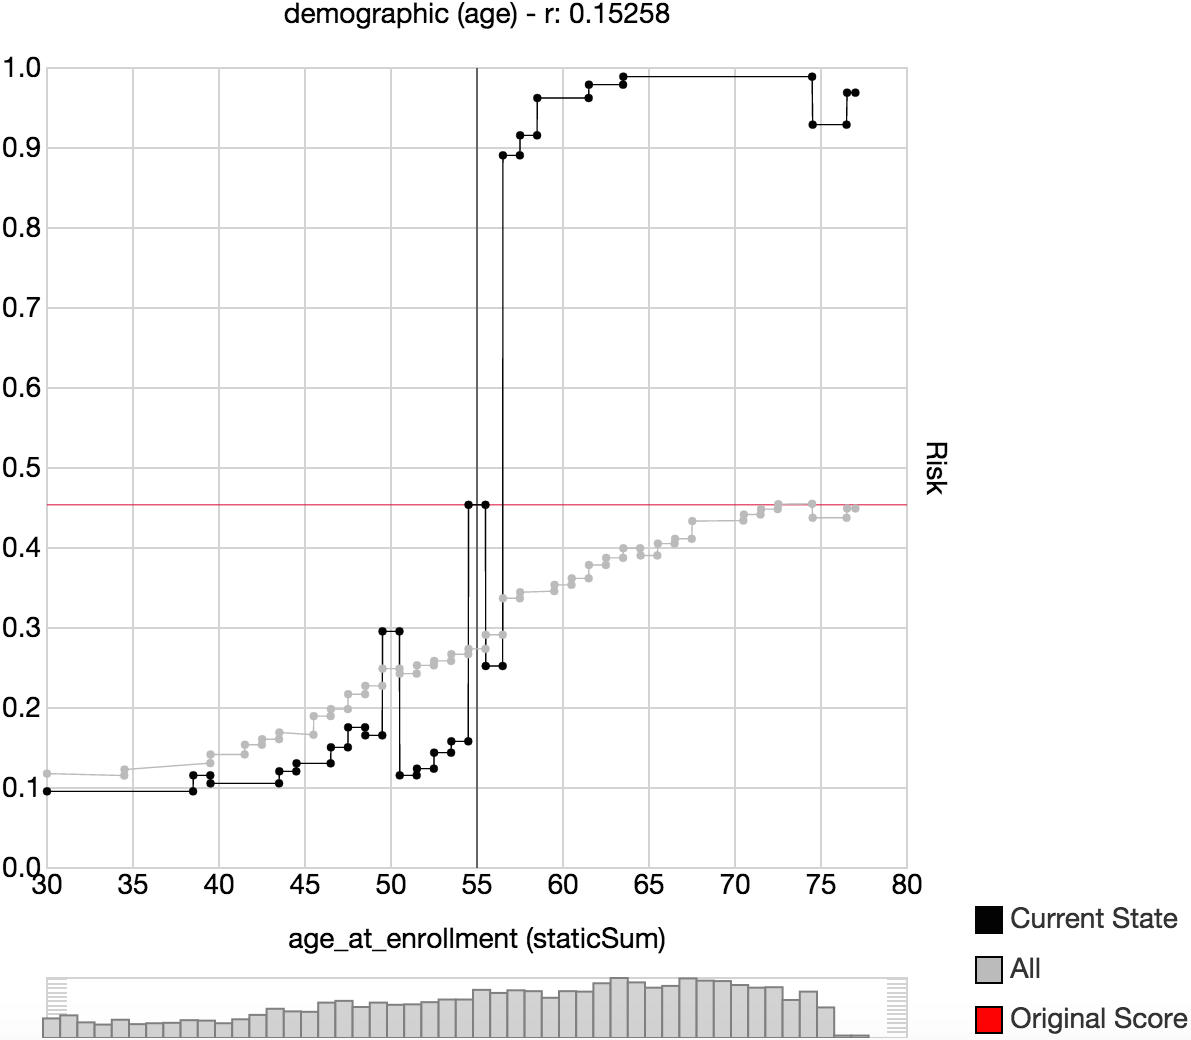
\includegraphics[width=0.8\linewidth]{prospector/compress_1} \\  \vspace*{0.2em} % 0.8 no vs
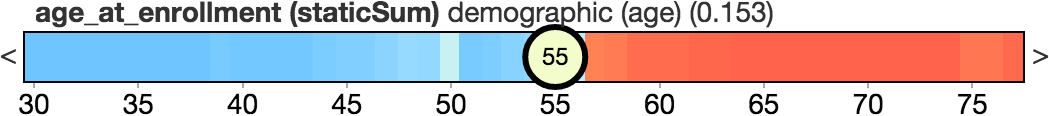
\includegraphics[width=0.9\linewidth]{prospector/compress_2} \\  \vspace*{0.5em} % 0.9 no vs
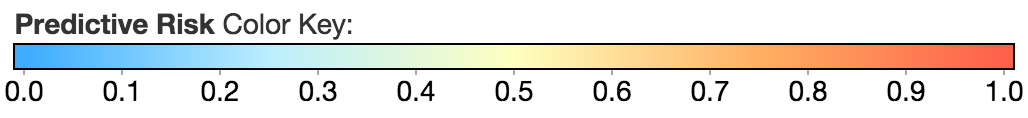
\includegraphics[width=0.7\linewidth]{prospector/color_scale} % 0.7
\caption[The same feature shown as line plot and partial dependence bar.]{
The same feature shown as line plot (top) and partial dependence bar (middle).
Color indicates the predicted risk for the outcome.
The color mapping is shown at the bottom.
}
\label{figs:compress}
\end{figure}

\subsubsection{Partial Dependence Bars}
In order to increase interactivity, encourage exploration, and display a larger number of features at once, we use a novel visual encoding, \emph{partial dependence bars}, a color bar representation of a partial dependence plot, shown in Figure~\ref{figs:compress}. The horizontal axis of a partial dependence bar represents the range of values of a feature, and the color at a given position represents the predicted risk for that value.  Color is mapped to a three-point color scale, where blue represents low risk, yellow represents medium risk, and red represents high risk.  As these bars are meant to aid local inspection, the current feature value of the datapoint being inspected is positioned along the horizontal axis and annotated as a circular label.  Users can drag this circular label left or right to inspect how changes in the feature value affect the predicted risk as well as the local partial dependence of other features.

\subsubsection{Local Feature Importance}
The fourth novel contribution of our research is a technique to simplify the
exploration of the predicted risk space by automatically finding features where a small change in value yields a significantly large change on the predicted risk.

While manipulating values of specific features allows users to test hypotheses on how features of interest may impact the prediction, if users wish to simply understand how to most impact the prediction, manipulating features one-by-one to test impact is an inefficient process.  Instead, \prospector can employ local feature importance, a novel technique that computes the impact of a given feature on the model according to the current values.  This localized feature importance comes in two different flavors: as a feature importance number and as actual suggestions for value changes.

A straight-forward way to define a localized importance of features is to look at the range of possible
predicted risks the feature can create starting from the given data point.
Formula (\ref{eq:importance}) computes the local importance $I$ of a given feature $f$ for the given feature
vector $p$. It sums up the entirety of changes in outcomes for all values $v$ for feature $f$.
The outcome changes are weighted by $\omega$ the likelihood of changing the value from $p_f$ to $v$.
$p^{\ast}$ is the modified feature vector where its value for $f$ is set to $v$ and $pred$ is the prediction function.

\begin{equation}
I_{f}(p) = \int_{-\infty}^{\infty}
\left[ pred(p^{\ast}) - pred(p) \right] \; \omega(v, \, p_f) \; dv
\label{eq:importance}
\end{equation}%
\[
\text{with}\; p^{\ast}_{f} = v \;\text{and}\; p^{\ast}_{g} = p_{g} \;\text{for}\; g \neq f
\]\[
\omega(v, \, p_f) = \frac{1}{\sigma_f \sqrt{2\pi}}
\exp \left( -\frac{(v - p_f)^2}{2\sigma_f^2} \right)
\]

In order for different features to be comparable, $\omega$ takes the distribution of values in the input data
into account. In features with a high spread, a larger change is more likely than in a feature with a narrow value range.
We model the likelihood of the change using a normal distribution with the reference value $p_f$ as mean and the
standard deviation $\sigma_f$ of the observed values of $f$ as standard deviation.
Ordering the features according to this local importance yields features that are likely to
decrease the predicted risk first, then features that have a low impact on the predicted risk,
and finally features that are likely to increase the predicted risk.

% \subsubsection{Local impact suggestions}
Instead of computing local feature importance for all possible changes, it is more
practically useful to compute the importance according to the most \emph{impactful} change for a feature.
An impactful change is the smallest change needed to have the largest change in the predicted outcome.
Note that this is different from the slope of the function since an impactful change
might be after a valley or ridge. Again, in order to have comparable
results, the distribution of values in the input data is taken into account.

\begin{equation}
\argmax_v \left[
s \; \left[ pred(p^{\ast}) - pred(p) \right] \; \omega(v, p_f)
\right]
\label{eq:impact}
\end{equation}

Formula (\ref{eq:impact}) finds the most impactful change of a feature.
$s$ is either $1$ or $-1$ depending on whether to search for the largest increase or decrease.
All other variables are the same as in Formula (\ref{eq:importance}).
The changes yielding the highest impact can be interpreted as suggestions for changing a data point.

\begin{figure}[t]
\centering
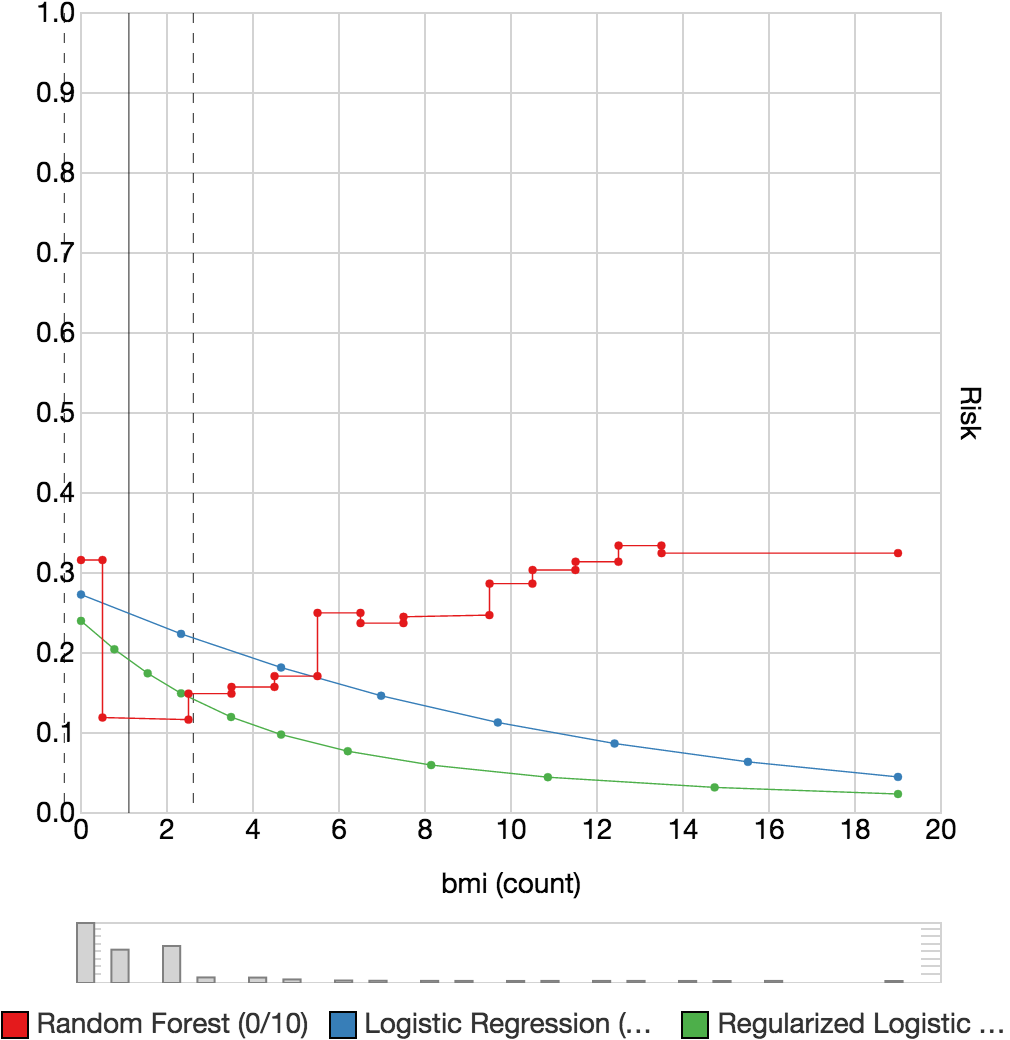
\includegraphics[width=0.7\linewidth]{prospector/cmp_bmi} % 0.8
\caption{
Comparison of three machine learning models on the number of measured BMI values.
The two regression models (logistic regression in blue and regularized logistic regression in green)
can express only a single slope (downwards or upwards) whereas the random forest in red can
model the strong decrease in predicted risk going from no BMI measures to one measure as well as
the later increase again if a patient has several BMI measures.
The random forest is more expressive, but the distribution of input values in the histogram below the plot hint the model might be overfitting as most of the observed values are 2 or less.
}
\label{figs:cmp_bmi}
\end{figure}


\subsubsection{Comparing Multiple Models}

%\joschi{TODO NaN values -- divergent models? there is not much to talk about this here...}

\prospector also supports plotting multiple models in the same plot.  As the input domain and the output range are the same across different machine learning
models on the same data,  partial dependence plots can also be used to compare multiple
models as shown in Figure~\ref{figs:cmp_bmi}.  This is useful for comparing the expressiveness of models and seeing which models are possibly under- or over-fitting the input data.

\subsection{Workflow}

In order to support the workflow of clinical researchers, as described above in the Motivation, \prospector's UI is organized into three main tabs: patient selection, patient inspection, and partial dependence plots.

\subsubsection{Patient Selection}

The patient selection tab allows users to find patients they may want to inspect, based on their ground truth (\eg, whether they actually had Diabetes) and their predicted risk (\eg, assessed likelihood by the predictive model of having the disease).  \prospector provides a visual summary of the patient population by providing a patient selection visualization. The visualization, as seen in Figure~\ref{figs:select}, consists of two columns dividing the population according to their ground truth
(case patients being those actually diagnosed with Diabetes and control patients being not).
Each column is then separated into bins of predicted probabilities in steps of $0.1$
which can be clicked to select the group of patients fitting those criteria.  For instance, if a case patient was predicted with a low risk score, that patient would appear in the top of the right column.  If a bin is too small to provide a clickable area, a box at the side of the column is displayed to allow choosing even small populations.  The selected population is then shown next to the visualization with the individual prediction results shown for each entry.

In order to get more details about patients before selecting, users can hover over a patient in the list and see a summary for the patient, as shown in Figure~\ref{figs:summary}.
In addition to the predicted risk and the ground truth, the interface shows the top 5 most impactful features, for both increasing and decreasing predicted risk, according to the local feature importance described above.  For each impactful feature, the original data value is shown as well as the suggested change and what the resulting predicted risk would be if such a change was made.  This summary provides a preview of how amenable a particular patient's predicted risk is to changing and which features are mostly responsible for their current predicted risk.

\subsubsection{Patient Inspection}

After users select a patient of interest, the UI switches to the
patient inspection tab with the selected patient's data loaded, as shown in Figure~\ref{figs:ui}.
All of the features' partial dependence bars are shown in a scrollable list, with the patient's feature values selected with circular labels.
Users can drag the circular label to change the value of any feature and see the predicted risk change in real-time.
Users can also select a feature and see the corresponding typical partial dependence plot of the feature.
In this plot the local partial dependence of the current patient is shown as
black curve and the global partial dependence of the whole population is shown
in gray. The partial dependence plot is also clickable and users can change the feature value here as well, changing the black vertical line that, in this plot, shows the current value.  

Users can change the order of the partial dependence bars by using the buttons at the top.  In addition to sorting by the feature weight and relevance as determined by the predictive model, users can also sort according to our local feature importance and impactful changes as described above.
If impactful changes are chosen as the order, the suggested changes to each feature are indicated with a white circular label in the partial dependence bar, shown on the bottom left of Figure~\ref{figs:ui}.

Often after analysts have inspected a particular patient, they may wish to find other patients similar to them to see how they react to the predictive model.  If users wish to find patients similar to the one they are inspecting, they can click on the ``Neighborhood" button and \prospector will automatically find the closest patients to the current set of values using feature-wise Euclidean distance.  This similar set of patients are then used as the population in the patient selection tab that users can navigate.

\subsubsection{Partial Dependence Plots}

If users wish to browse the global partial dependence plots of a feature of interest, they can navigate to the third tab.  Users can view multiple models at once by using a combo-box at the top of the user interface to select the models they wish to view in the plot.  Each selected model is assigned a unique color using a quantitative color scale, and a color-coded key is displayed beneath the plot.  If more than one model is selected, the red ``Avg. Score" helper line is not shown.  Users can also filter the global population to a subset population of interest by using a  predicted probability bin or the ``Neighborhood" of a patient in the patient selection tab. This alters the plot accordingly allowing for a more focused analysis for \eg, mispredicted patients, outliers, or patient neighborhoods.

\begin{figure}
\centering
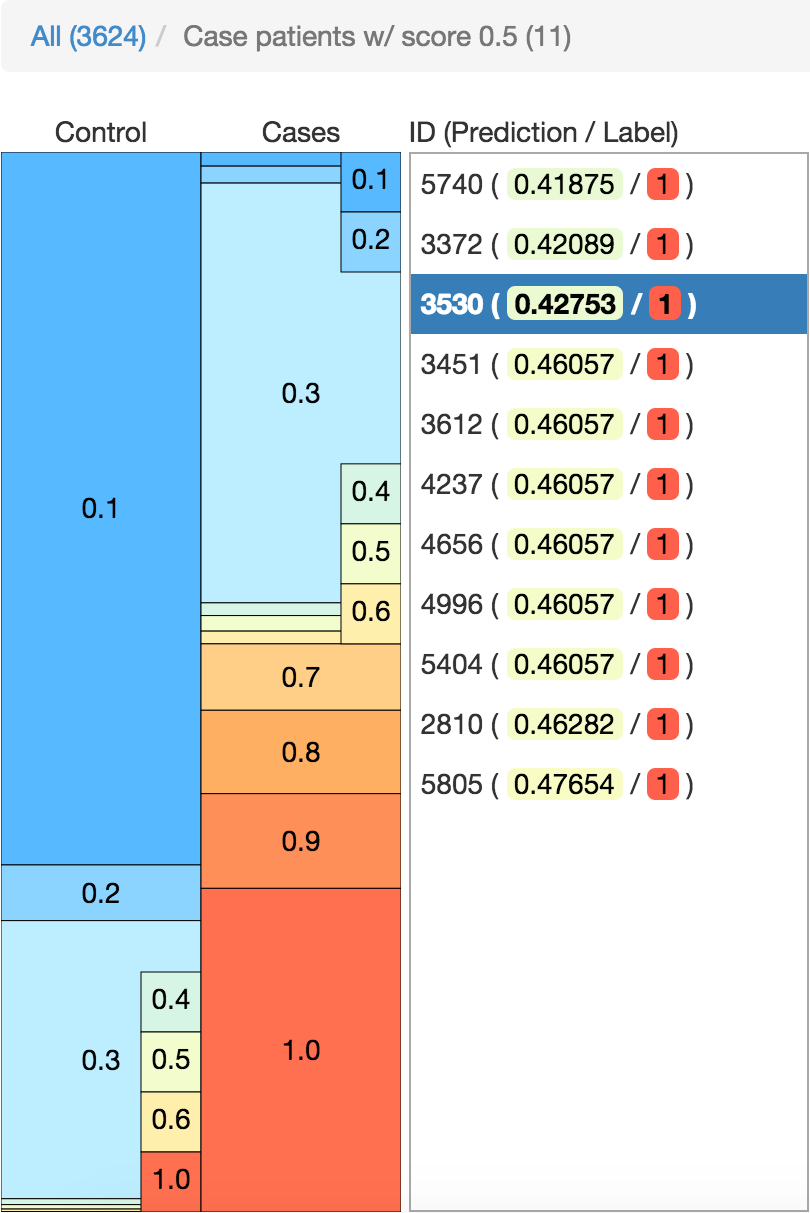
\includegraphics[width=0.5\linewidth]{prospector/patient_select} % 0.6
\caption[The interface for selecting a patient.]{
The interface for selecting a patient.
The left side shows the distribution of patients within different ranges of predicted risk.
The columns indicate the ground truth.
On the right side a list shows the patients of the currently selected range.
}
\label{figs:select}
\end{figure}

\begin{figure}[t]
\centering
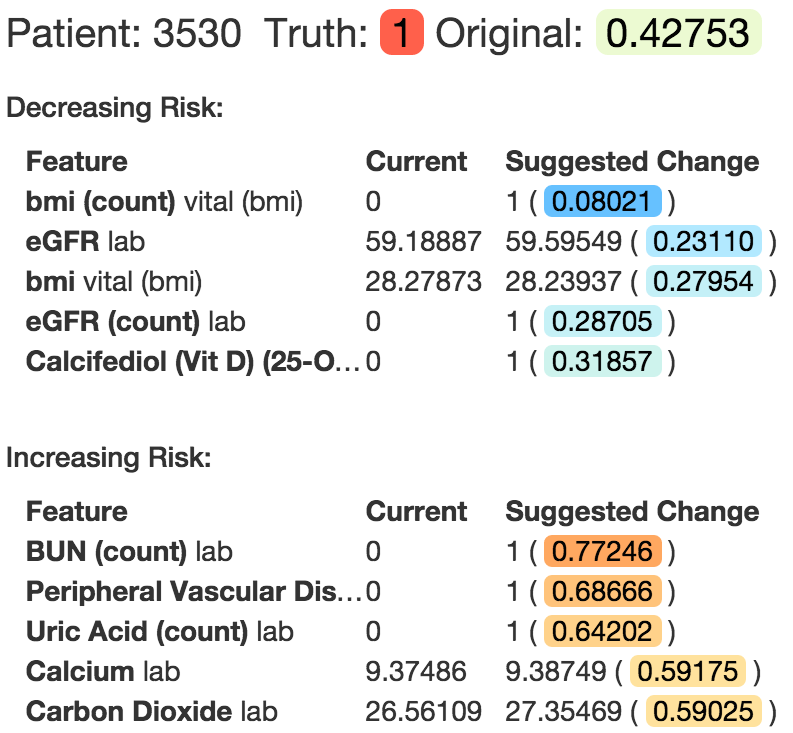
\includegraphics[width=0.5\linewidth]{prospector/patient_summary} % 0.7
\caption{
The summary of one patient. The header line indicates the patient id, the ground truth, and the predicted
risk.
For both decreasing and increasing the predicted risk the top 5 most impactful features are shown.
Each feature shows its current value and the suggested change with the highest impact along with how the predicted risk would change.
}
\label{figs:summary}
\end{figure}

\begin{figure}[t]
\centering
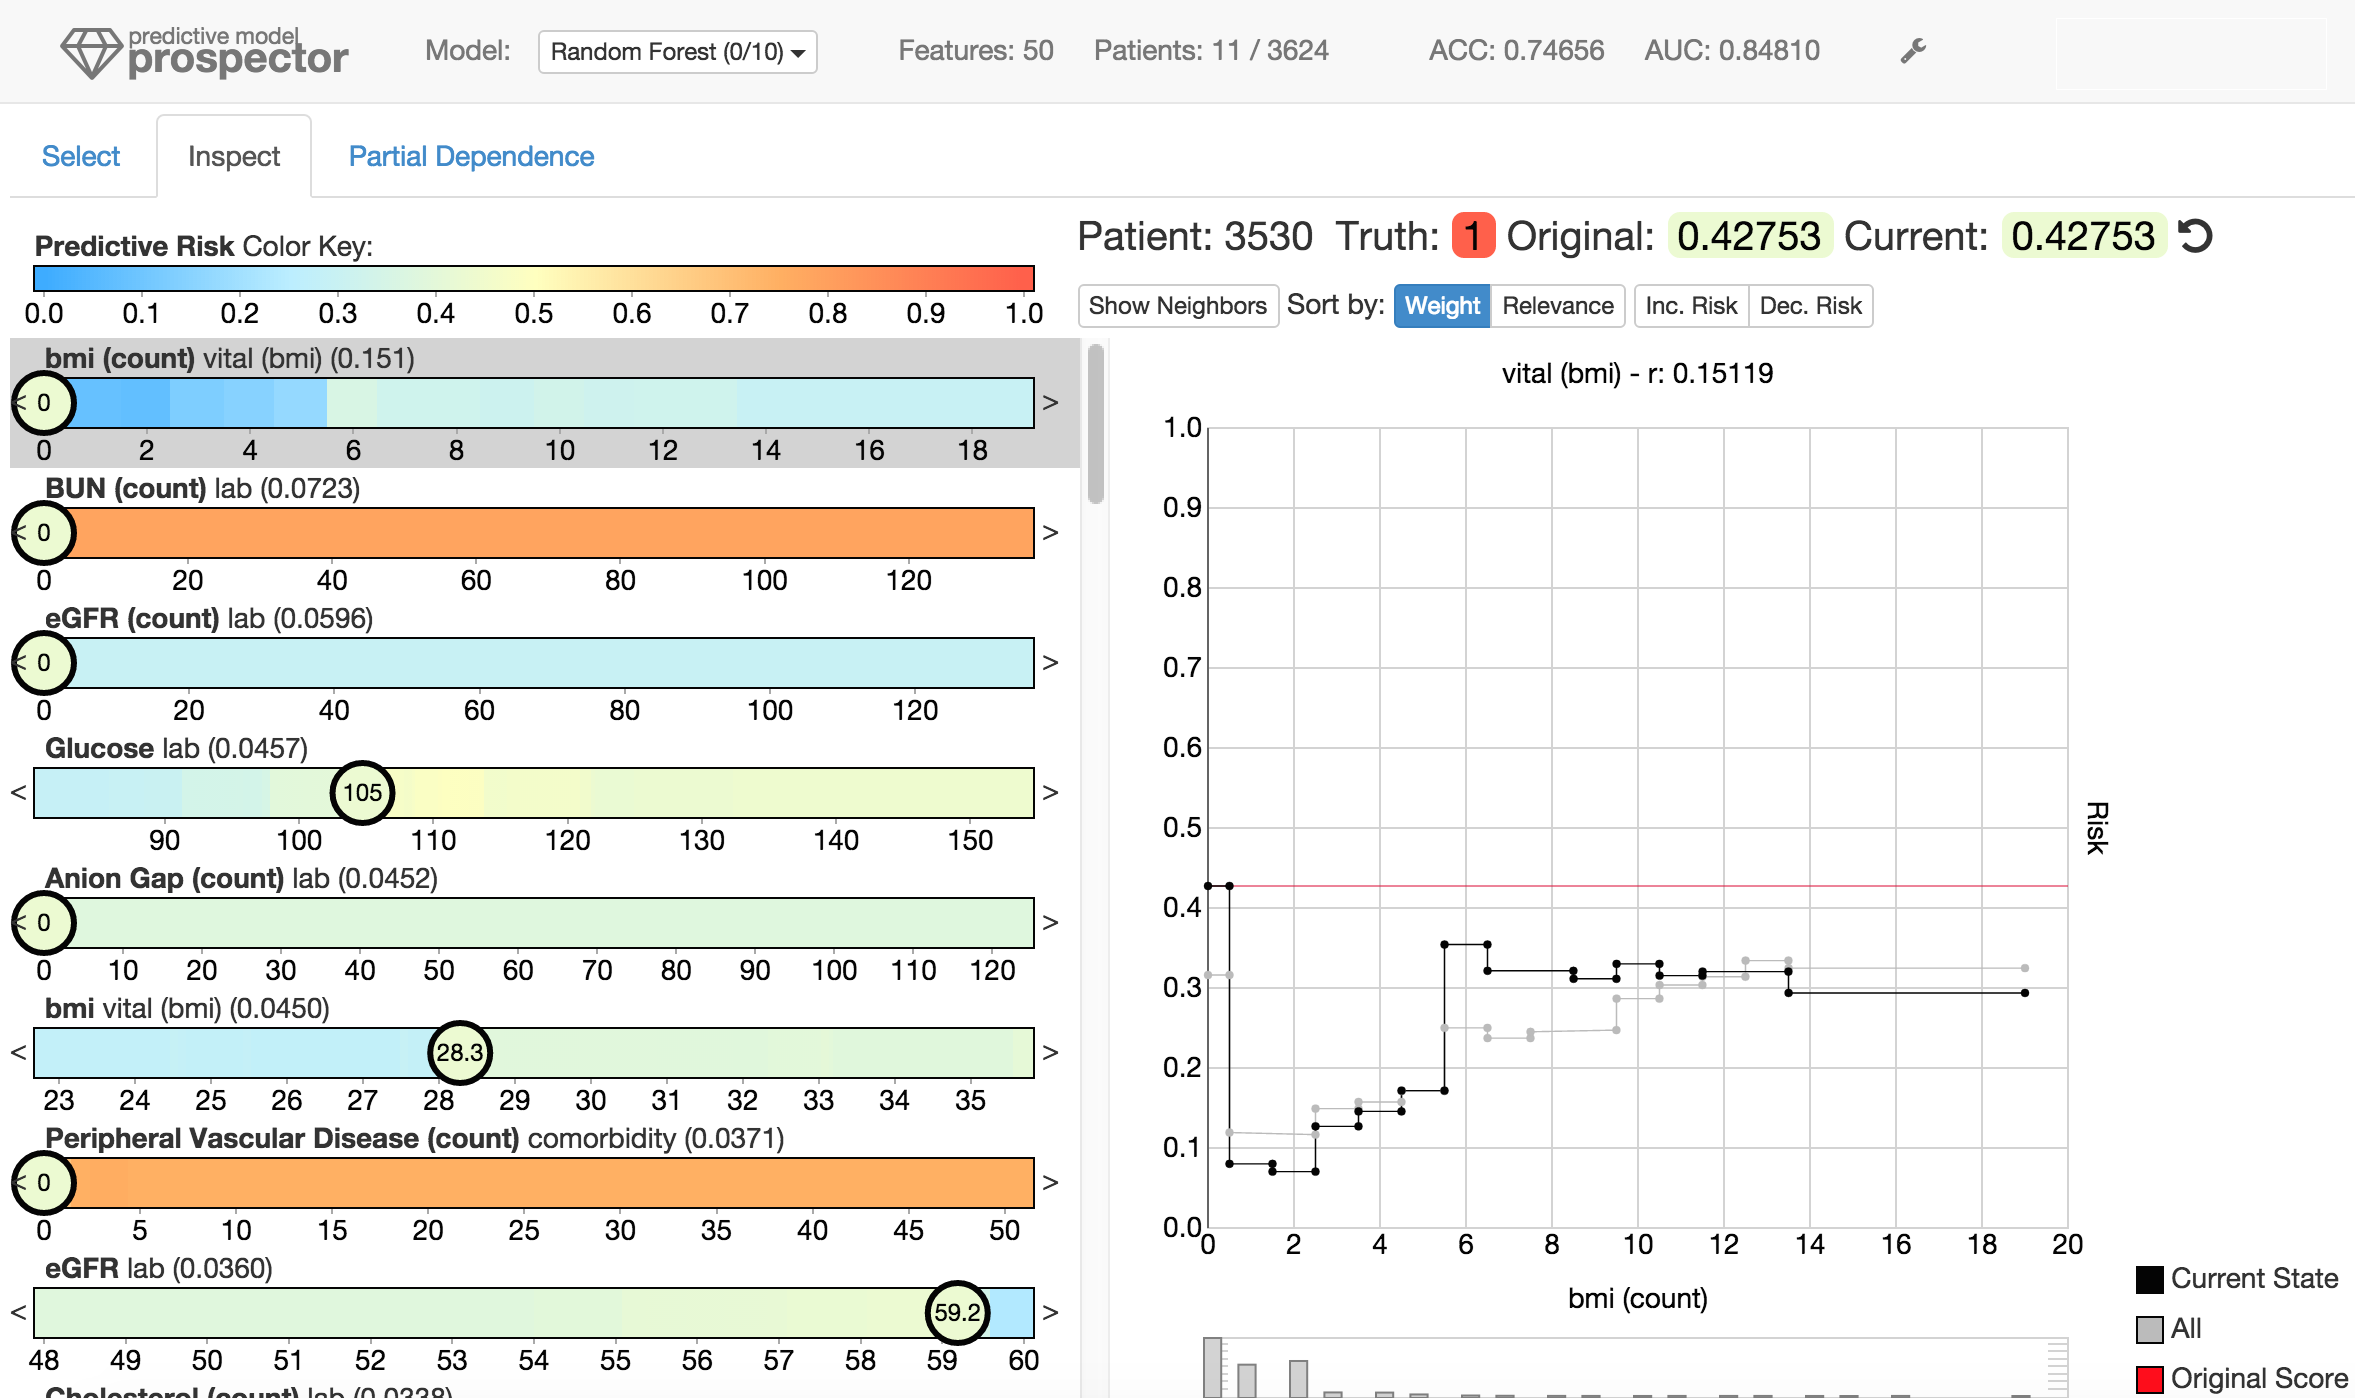
\includegraphics[width=0.8\linewidth]{prospector/ui_inspect} % 0.775
\\
\vspace*{0.75em} % 2
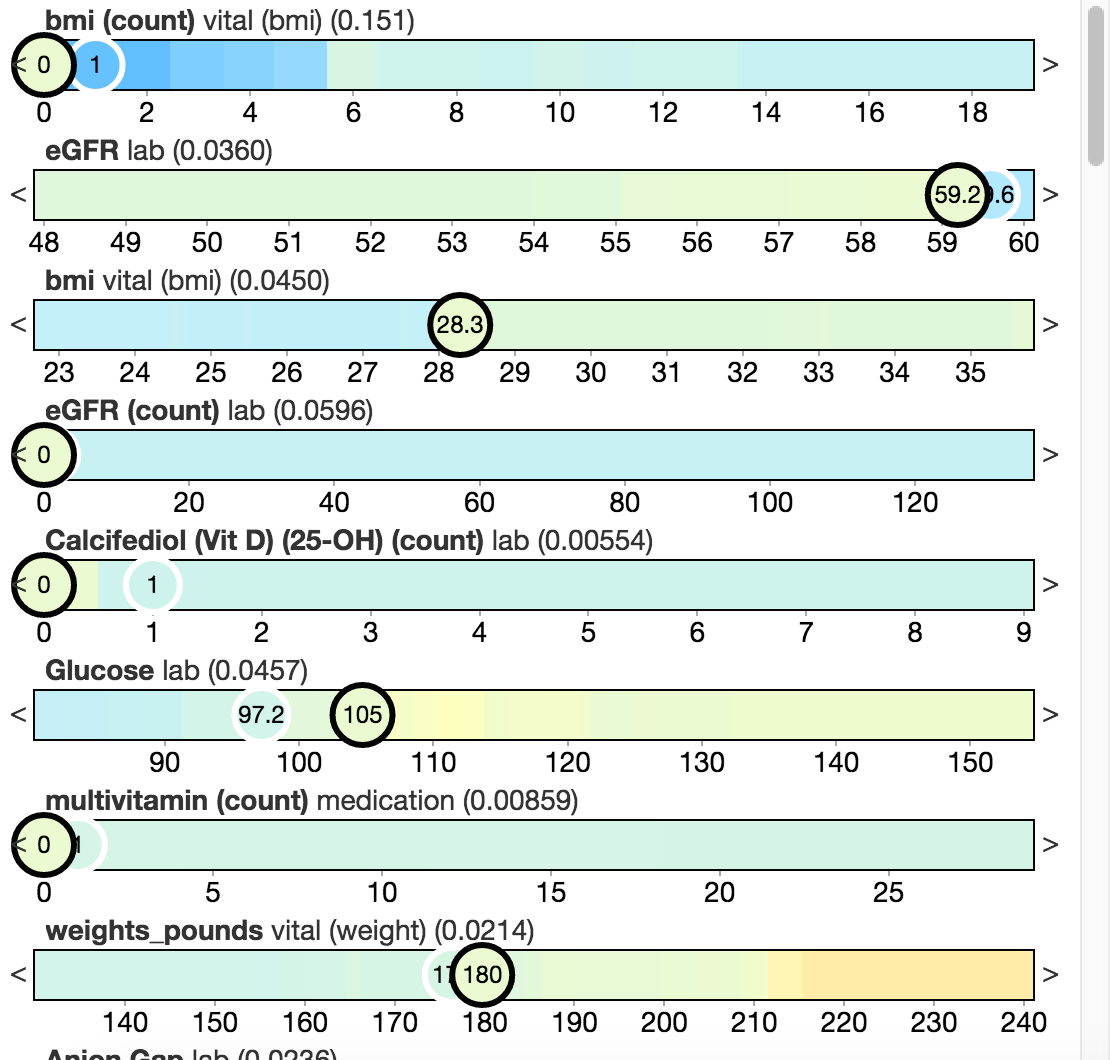
\includegraphics[width=0.3\linewidth]{prospector/ui_sugg} % 0.3
\hspace*{0.2\linewidth} % 18
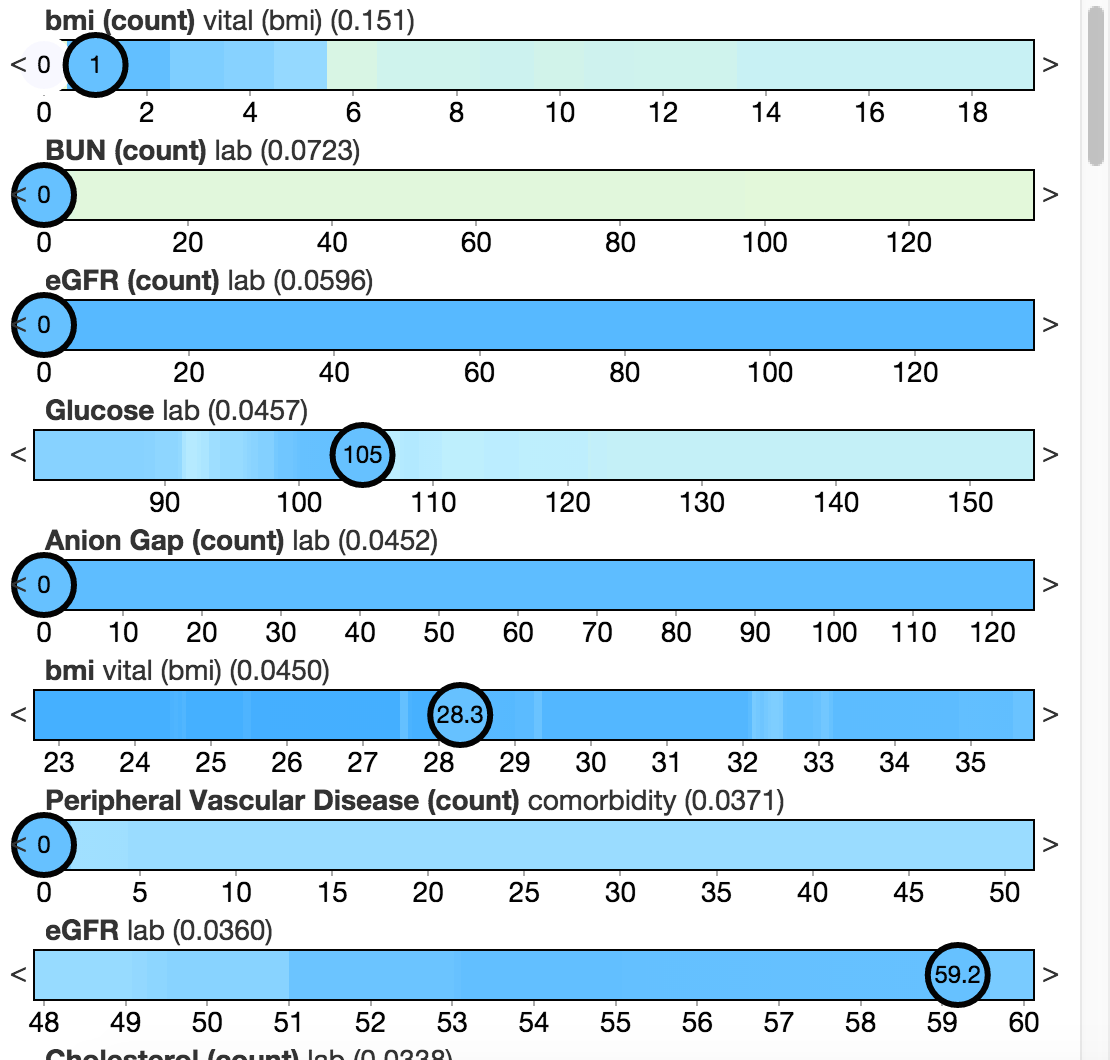
\includegraphics[width=0.3\linewidth]{prospector/ui_change} % 0.3
% \vspace*{1em}
\caption[The user interface of \prospector.]{
The user interface of \prospector is shown at the top.
The bottom left shows suggestions on what changes (white circles) would decrease the
predicted risk the most.
The bottom right shows how the color plots change due to changing a value (namely changing the
bmi value from 0 to 1).
Fully white circles show the original value of the given patient.
}
\label{figs:ui}
\end{figure}

% !TEX root = ../prospector.tex

\section{Case Study: Predicting Diabetes}

In order to evaluate the utility of \prospector, we chose to conduct a case study utilizing a team of real data scientists building their own predictive models on their own real-world datasets to demonstrate its effectiveness at reaching insights in practice. There is a growing belief in the visualization community that traditional evaluation metrics (e.g. measuring task time completion or number of errors) are often insufficient to evaluate visualization systems \cite{bertini_summaries:_2011,plaisant_challenge_2004,shneiderman_strategies_2006}. Using the evaluation methodology developed by Perer and Shneiderman \cite{perer_integrating_2008}, we conducted a 4-month long-term case study with a team of five data scientists interested in using predictive modeling on a longitudinal database of electronic medical records. The research team is interested in building a predictive model to predict if a patient is at risk of developing diabetes using a database of 4,000 patients from a major hospital in the United States.  Due to sensitive data agreements, this team wished to remain anonymous.  

The initial phase of the case study involved understanding the data scientists' current tools and needs.  They presented their typical results after building predictive models, sharing stories of success when their stakeholders were pleased, as well as examples of less successful results when their stakeholders demanded answers they couldn't provide with existing tools.  Their use cases and experiences shaped the design and requirements of the tool.

After the tool was developed, there were bi-weekly meetings with the data science team in which we discussed the current interface and identified shortcomings of the interface, necessary UI enhancements, and components that were not worth developing further.  Some of the elements originally proposed turned out not to be useful, such as overlaying distributions of risk in the partial dependence plots or using ICE plots \cite{goldstein14}.  However, focusing the meetings on examining the team's predictive models together using \prospector allowed us to determine which elements helped improve both the models and their comprehension of the models.

\subsection{Understanding Model Classes}

Initially, the data scientists were unsure which type of predictive models to build.  Although they had used simpler models in the past, such as decision trees and logistic regression, they were eager to use random forest models due the promise of higher accuracy but were worried about how interpretable the results would be.
After building models using both logistic regression and random forests, they were curious to use partial dependence plots to understand the trade-offs of both approaches. An example of such trade-offs can be seen in Figure~\ref{figs:cmp_bmi}, which is a partial dependence plot of two logistic regression models and one random forest. Interestingly, for this feature (which refers to the number of times patients got their BMI recorded), the model types disagree substantially for higher values in the plot. This is surprising since the inspected feature is most important for all models and
all models perform equally well using standard statistics like accuracy or AUC.

While all three models have a decrease in average predicted risk when the count goes from 0 to 2, the logistic regression models continue to trend downward.  However, the random forest model (in red), illustrates the predictive risk increases as the count gets higher than two.  The data scientists were surprised to learn how differently the model classes treated this feature, but using the tool, they were able to devise a two-fold explanation.  On one hand, logistic regression models are not expressive enough to model the late increase after the initial drop, as logistic regression models are bound by a single curve.  On the other hand, most of the observed data points of the feature are zero, one, and two while the higher values occur extremely rare, as the histogram below the plot clearly illustrates.  This led the data scientist team to question whether to model everything as precisely as possible or using a simpler model for the sake of generality.

\subsection{Unexpected Effects of Data Imputation}

Due to limitations of their database, many of the patients were missing Glucose lab test results.  During the feature construction phase, the team made a decision that in order to work around the missing values, each patient who did not have a value would be given the average observed value of all other patients.  This imputation technique is popular among predictive modelers, as simply removing all patients without such data would make the data quite small.  However, once the data science team began to explore the Glucose feature in the tool, as shown in Figure~\ref{figs:sampling}, they began to realize the dramatic effects their imputation strategy can have.  Due to the imputation, patients that are either cases or controls often have the same lab test values which increases the noise of the predicted risk.  The partial dependence plot illustrates that, as noise increases, the predicted probability gets closer to the population average leading to a valley in the machine learning model.  Exploring this feature in \prospector suggested that a better strategy for handling missing values would be needed to overcome this problem.

\subsection{The Need for Localized Inspection}

Discussions in bi-weekly interviews also led to the development of the localized inspection of patients
which aims to answer the following questions:
\begin{enumerate}
\item What impact does a feature have on an actual patient?
\item Does the model behave correctly on a case-to-case basis?
\item What are the most important features for a given patient?
\item Why are certain patients not being accurately predicted?
\item Can we identify high impact actionable features?
\end{enumerate}

The last question about identifying actionable features was of particular importance to the data science team.  They were interested to know if the model could be used to learn features that could be acted upon by the patients or their doctors to reduce the risk of diabetes.  However, the data science team were disappointed to learn, via \prospector, that many of the highest ranking features were not actionable.  For instance, some of the most predictive features for a high risk of diabetes involved having a high count of the number of lab tests.  Informing patients to get fewer lab tests would likely not correlate to lower risk of diabetes.  Instead, these lab test counts were likely a proxy for other features that correlated to more complicated or more sickly patients seeing their doctors more regularly and thus getting more lab tests.  Other demographic features that were highly predictive, like age, simply have no intervention as well.  The data science team then reconsidered which features should be a part of the predictive model, by creating features that are actionable and omitting others.  Of course, the model cannot know this by itself -- no matter what sophisticated feature selection algorithms are used -- so the access \prospector provides is critical for this process.

\subsection{Impact into Data Scientists' Workflow}

In addition to learning new insights about their predictive models, the tool also impacted the team's workflow.  Prior to \prospector, after each new predictive model was built, a data scientist would manually generate a set of reports describing the model.  Typically, this would involve exporting a list of the model's top features and their weights, and generating a bar chart for the other team members to review.  They would present these bar chart summaries during review meetings and discuss if the model seemed sensible enough.  If they believe the list of features made sense, they would then present this chart to their stakeholders.  If it didn't, they would brainstorm how to improve the predictive model (such as changing the classification or feature selection algorithms) and then repeat this process.  While this manual approach led to the deployment of predictive models in the past, many iterations were required and understanding impactful values of features were rarely considered.

Once \prospector was integrated into their workflow, many of these shortcomings were overcome.  No longer did a data scientist need to generate a set of manual reports.  Instead, the predictive model can be loaded into the tool directly.  Since the tool is interactive, it also allows the team to ask questions that may have not been considered when static charts were created.  The tool also allowed them to ask questions beyond the top features that contributed to the models.  They could ask more patient-centric questions such as ``Why is this patient not being classified correctly?" by drilling down to incorrectly predicted patients and exploring the most impactful features for them. Beyond exploration, \prospector was also used to communicate models to the stakeholders, which allowed stakeholders to ask questions and see the results in real-time.  This rapid feedback helped gain support for deploying predictive models in future projects.  As a result of these successes, \prospector is now a part of their predictive modeling workflow and is used for other work than predicting the onset of diabetes.

% R2 wanted more details about the how
%   Prospector was used with respect to the other tools the data science team
%   was already using, how Prospector impacted the larger organization, and
%   how did it get used by other stakeholders mentioned

%  We were pleased that all
% of the reviewers appreciated our 4-month long deployment, but we do agree
% more details can be provided. In the revision, we will describe how the
% deployment led to an improved design, as some prototypes originally
% considered turned out to be not useful for their tasks (shaded areas
% showing distributions in risk, ICE plots). In addition, we will describe
% how the tool fit into their workflow and also stories of how it impacted
% the stakeholders (the participants actually used our visualization and
% interactive demos to communicate the models to their executives and
% scientists, which gained support for predictive modeling in new
% projects). Prospector is now part of their workflow, and they are using
% it for other modeling work, including domains beyond diabetes


%\adam{Possible second story:  Better understand patients that weren’t being classified correctly}

% !TEX root = ../prospector.tex

\section{Conclusion and Discussion}

In this paper, we demonstrated how the design and implementation of an interactive visual analytics system,
\prospector, can help data scientists assess the interpretability and actionable insights of trained predictive models. \prospector accomplishes this by supporting interactive partial dependence diagnostics for understanding how features affect the prediction overall by featuring novel visual representations, sampling strategies, and support for comparing multiple models.  Furthermore, \prospector supports localized inspection so data scientists can understand how and why specific instances are predicted as they are.  With support to interactively tweak feature values and see how the prediction responds, as well as finding the most impactful features using a novel local feature importance metric, data scientists can interact with models on a deeper level than possible with common tools.  Finally, we presented a case study, in the spirit of \#chi4good, which involved a team of data scientists using \prospector  to improve predictive models for detecting the onset of Diabetes.  Their extended use of the tool led to better predictive models, as well as better communication of their models to their stakeholders.

% In this paper we demonstrated how \systemname can be used to analyze, compare, and improve
% machine learning models.
% Furthermore, we took the concept of Partial Dependence and applied it to single cases
% enabling ``what-if" scenarios which in turn can be used to retrieve a localized importance
% of input features and suggestions for actionable changes which impact the predicted outcomes.

% that is rarely the case.
% Consider, for example, our system suggesting the change of a patient's Glucose value.
% This change can be achieved using medication or a life-style change but it would thus most likely
% change other values of the patient's input vector as well.

Despite the novel features of \prospector and its successful case study, there is still much future work to continue to give users full comprehension of predictive models. \prospector relies on partial dependence for one input feature at a time, but this approach relies on the orthogonality of input features.  However, in real-world data, this is not often the case, as features may be correlated.  \prospector can only model changes along one axis at a time as it cannot take correlations or influences between features into account.
We plan to address this limitation in future work by modeling valid sets of instances and visualizing how
they react to changes in one or more features.  Another limitation is that \prospector was built to view predictive models after they had been built using users' own predictive modeling pipeline of choice.  However, this flexibility limits the ability for users to directly impact their predictive models based on insights reached during exploration. Also, \prospector can only handle single-class predictions, but we plan to extend this functionality to multi-class predictions in the future.
Our future work also intends to integrate \prospector more directly into the predictive modeling pipeline so users can directly modify features for feature construction and feature selection and see how their models improve in a single user interface.  Despite these limitations, providing users with advanced visual tools to inspect black-boxes of machine learning shows great promise and helps users comprehend and retain control of their predictive models without sacrificing accuracy.

% \balance{}

% \bibliographystyle{SIGCHI-Reference-Format}
% \bibliography{prospector}
% \balance

% \end{document}

%%% Local Variables:
%%% mode: latex
%%% TeX-master: t
%%% End:
